\documentclass[a4paper,11pt]{article}
\usepackage[T1]{fontenc}
\usepackage[utf8]{inputenc}
\usepackage{lmodern}
\input GetPackages

\title{MICE Target Simulation}
\author{Tom Lord, Paolo Franchini}

\begin{document}

\maketitle
\tableofcontents

\begin{abstract}
Simulation of the pion production coming out from the MICE target using the MARS simulation software and implementation of this simulation into the MICE Monte Carlo software.
\end{abstract}

\newpage

\section{Motivation}

Non trivial discrepancies in the data versus Monte Carlo comparison have justified the necessity to reconsider the pions momentum distribution used as primary input of the MICE Monte Carlo.
The former model consisted in a fit done with three Gaussian of a pion distribution produced in 2008 with a earlier version of the MARS simulation software. Lack of documentation on this first study made hard to evaluate the goodness of the model that shows a peculiar hard cut in the distribution.

The MICE target has been described in its major components using the MARS simulation software.
\section{The MICE target in the ISIS proton beam}

\*Brief description of the MICE target.\\*\
The MICE target operates parasitically on protons undergoing acceleration within the ISIS synchrotron, dipping into the low-density halo of the beam on selected pulses just prior to their extraction, with an ~1 Hz frequency. It is designed as a bored TiAl cylinder with inner radius 2.275 cm and outer radius 2.975 cm. The resulting thickness of material for proton collisions is significantly lower than one interaction length, giving an approximate interaction probability of x~~x. As a result of this,very large numbers of proton collisions are required for sufficient statistics. 

\*ISIS proton beam: energy, dimension, position...*\
The ISIS synchrotron circulates two beam bunches of approximately 1.4E13 protons each per cycle, with these undergoing close to 10,000 revolutions before extraction in a circulation time of 10ms. This proton beam undergoes beam-size shrinking between radii of ~67mm and 48mm during it's acceleration through the synchrotron, and hence proton collision energy and beamwidth will both vary in time with respect to the initial ISIS proton injection trigger, as well as due to small field fluctuations. In practice this means the target undergoes proton collisions of between 650MeV and 800MeV collision energy. Furthermore due to the field changes in the synchrotron, the ISIS beam often drifts from the well-defined beam center, such that the beam centre displacement (BCD) figure recorded is only a nominal value. 

As noted in (target-ref) the target 

\section{MARS simulation}

The design of the MICE target, in particular the surrounding structure, is defined as in~Fig.~\ref{fig:MARSvent}. The presented design has been based on schematics (ref) and surveys (refs). The MICE beamline is orientated at 25 deg with respect to the ISIS beamline section where the target is located.

Numerous features have been implemented in addition to the cylindrical bored-target structure from the previous model, including the rectangular beampipe shape and target window structure similarly oriented at 25 degrees toward the MICE beamline. 

\begin{figure}[t!]
  \begin{center}
    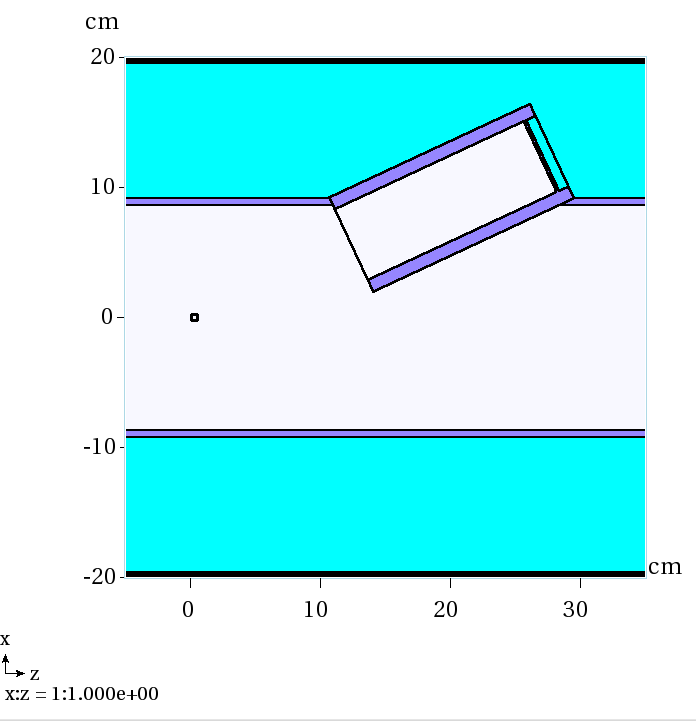
\includegraphics[width=1.0\columnwidth]{./figures/MARSv2TargetVent.png}
    \caption{Design of the target in the MARS simulation. ( require z=60cm?along the x-axis? ) }
    \label{fig:MARSvent}
  \end{center}
\end{figure}

\begin{figure}[t!]
  \begin{center}
    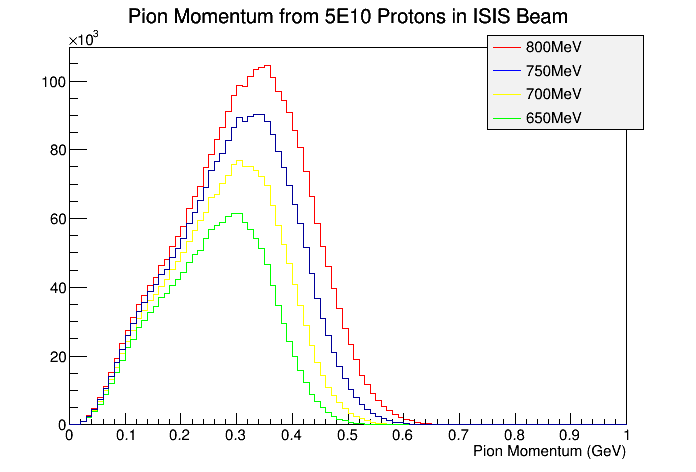
\includegraphics[width=1.0\columnwidth]{./figures/PiMomentum.png}
    \caption{}
    \label{fig:PiMomentum}
  \end{center}
\end{figure}


\section{MAUS simulation}

The Monte Carlo in MICE is produced in a two-step process. In the first step a pion beam is produced according to an initial momentum distribution and is propagated using G4BL up to the bending dipole D2. After this point MAUS takes over propagating the particles (pions, muons and electrons coming from decays) through the remaining part of the beamline up to the EMR, passing through the cooling channel, according to the geometry and run selected to be simulated. 

\subsection{Monte Carlo and data comparison}

Few figure of merits have been considered: time of flight of the particles between TOF0 and TOF1 and momentum distribution of pions and muons in the upstream tracker at station 5.
Simulations have been produced for 140, 200 and 240 MeV/c nominal pionic beams.

\section{Luminosity monitor?}
\textit{Shall we produce with MARS scattered protons and compare the flux in the LM position (-25 deg, 10 meters away) with the measured one?} 

\section{Conclusions}

\begin{thebibliography}{9}
\bibitem{mars} https://mars.fnal.gov/
\bibitem{micenote216} MICE note \#216, http://mice.iit.edu/micenotes/public/pdf/MICE0216/MICE0216.pdf
\bibitem{micenote242} MICE note \#242, http://mice.iit.edu/micenotes/public/pdf/MICE0242/MICE0242.pdf
\bibitem{beampipesurvey1} ISIS Survey Drawing, \#1-SI-6305-031-01-D
\bibitem{beampipesurvey2} ISIS Survey Drawing, \#1-SI-6305-031-02-C
\bibitem{beampipesurvey3} ISIS Survey Drawing, \#1-SI-6305-031-03-C

\end{thebibliography}

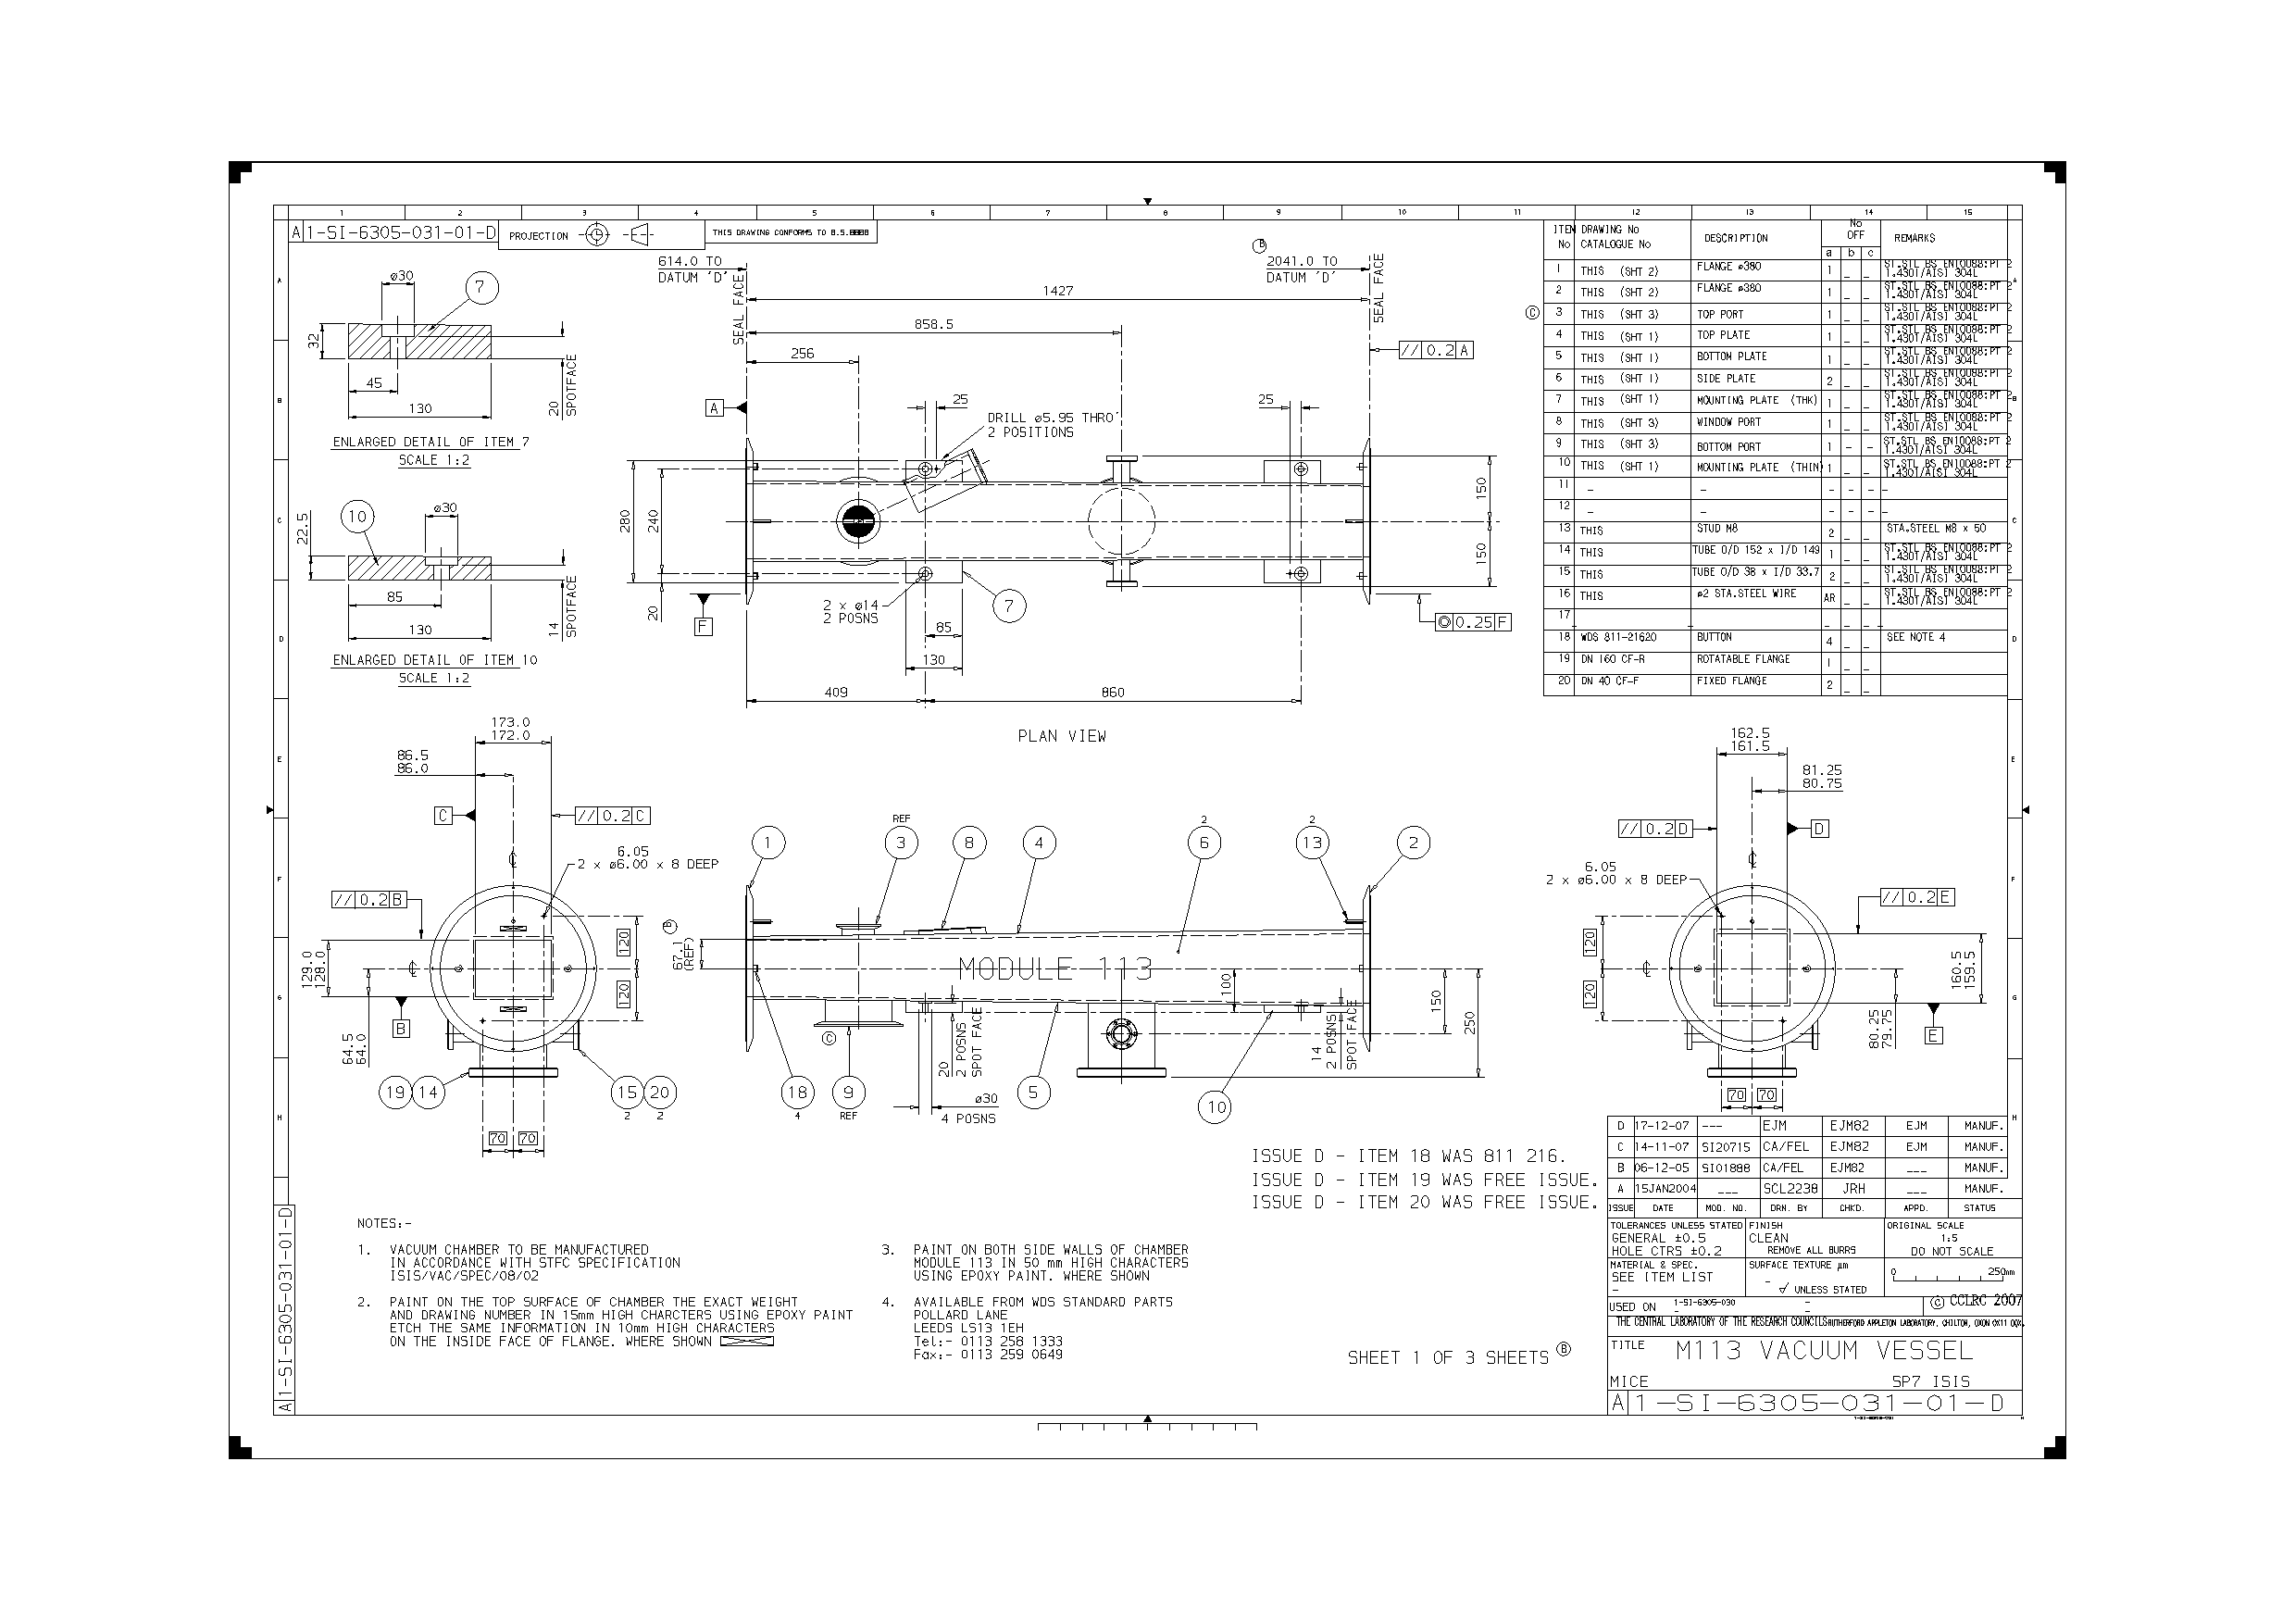
\includepdf{./figures/BeampipeSurvey1.pdf}
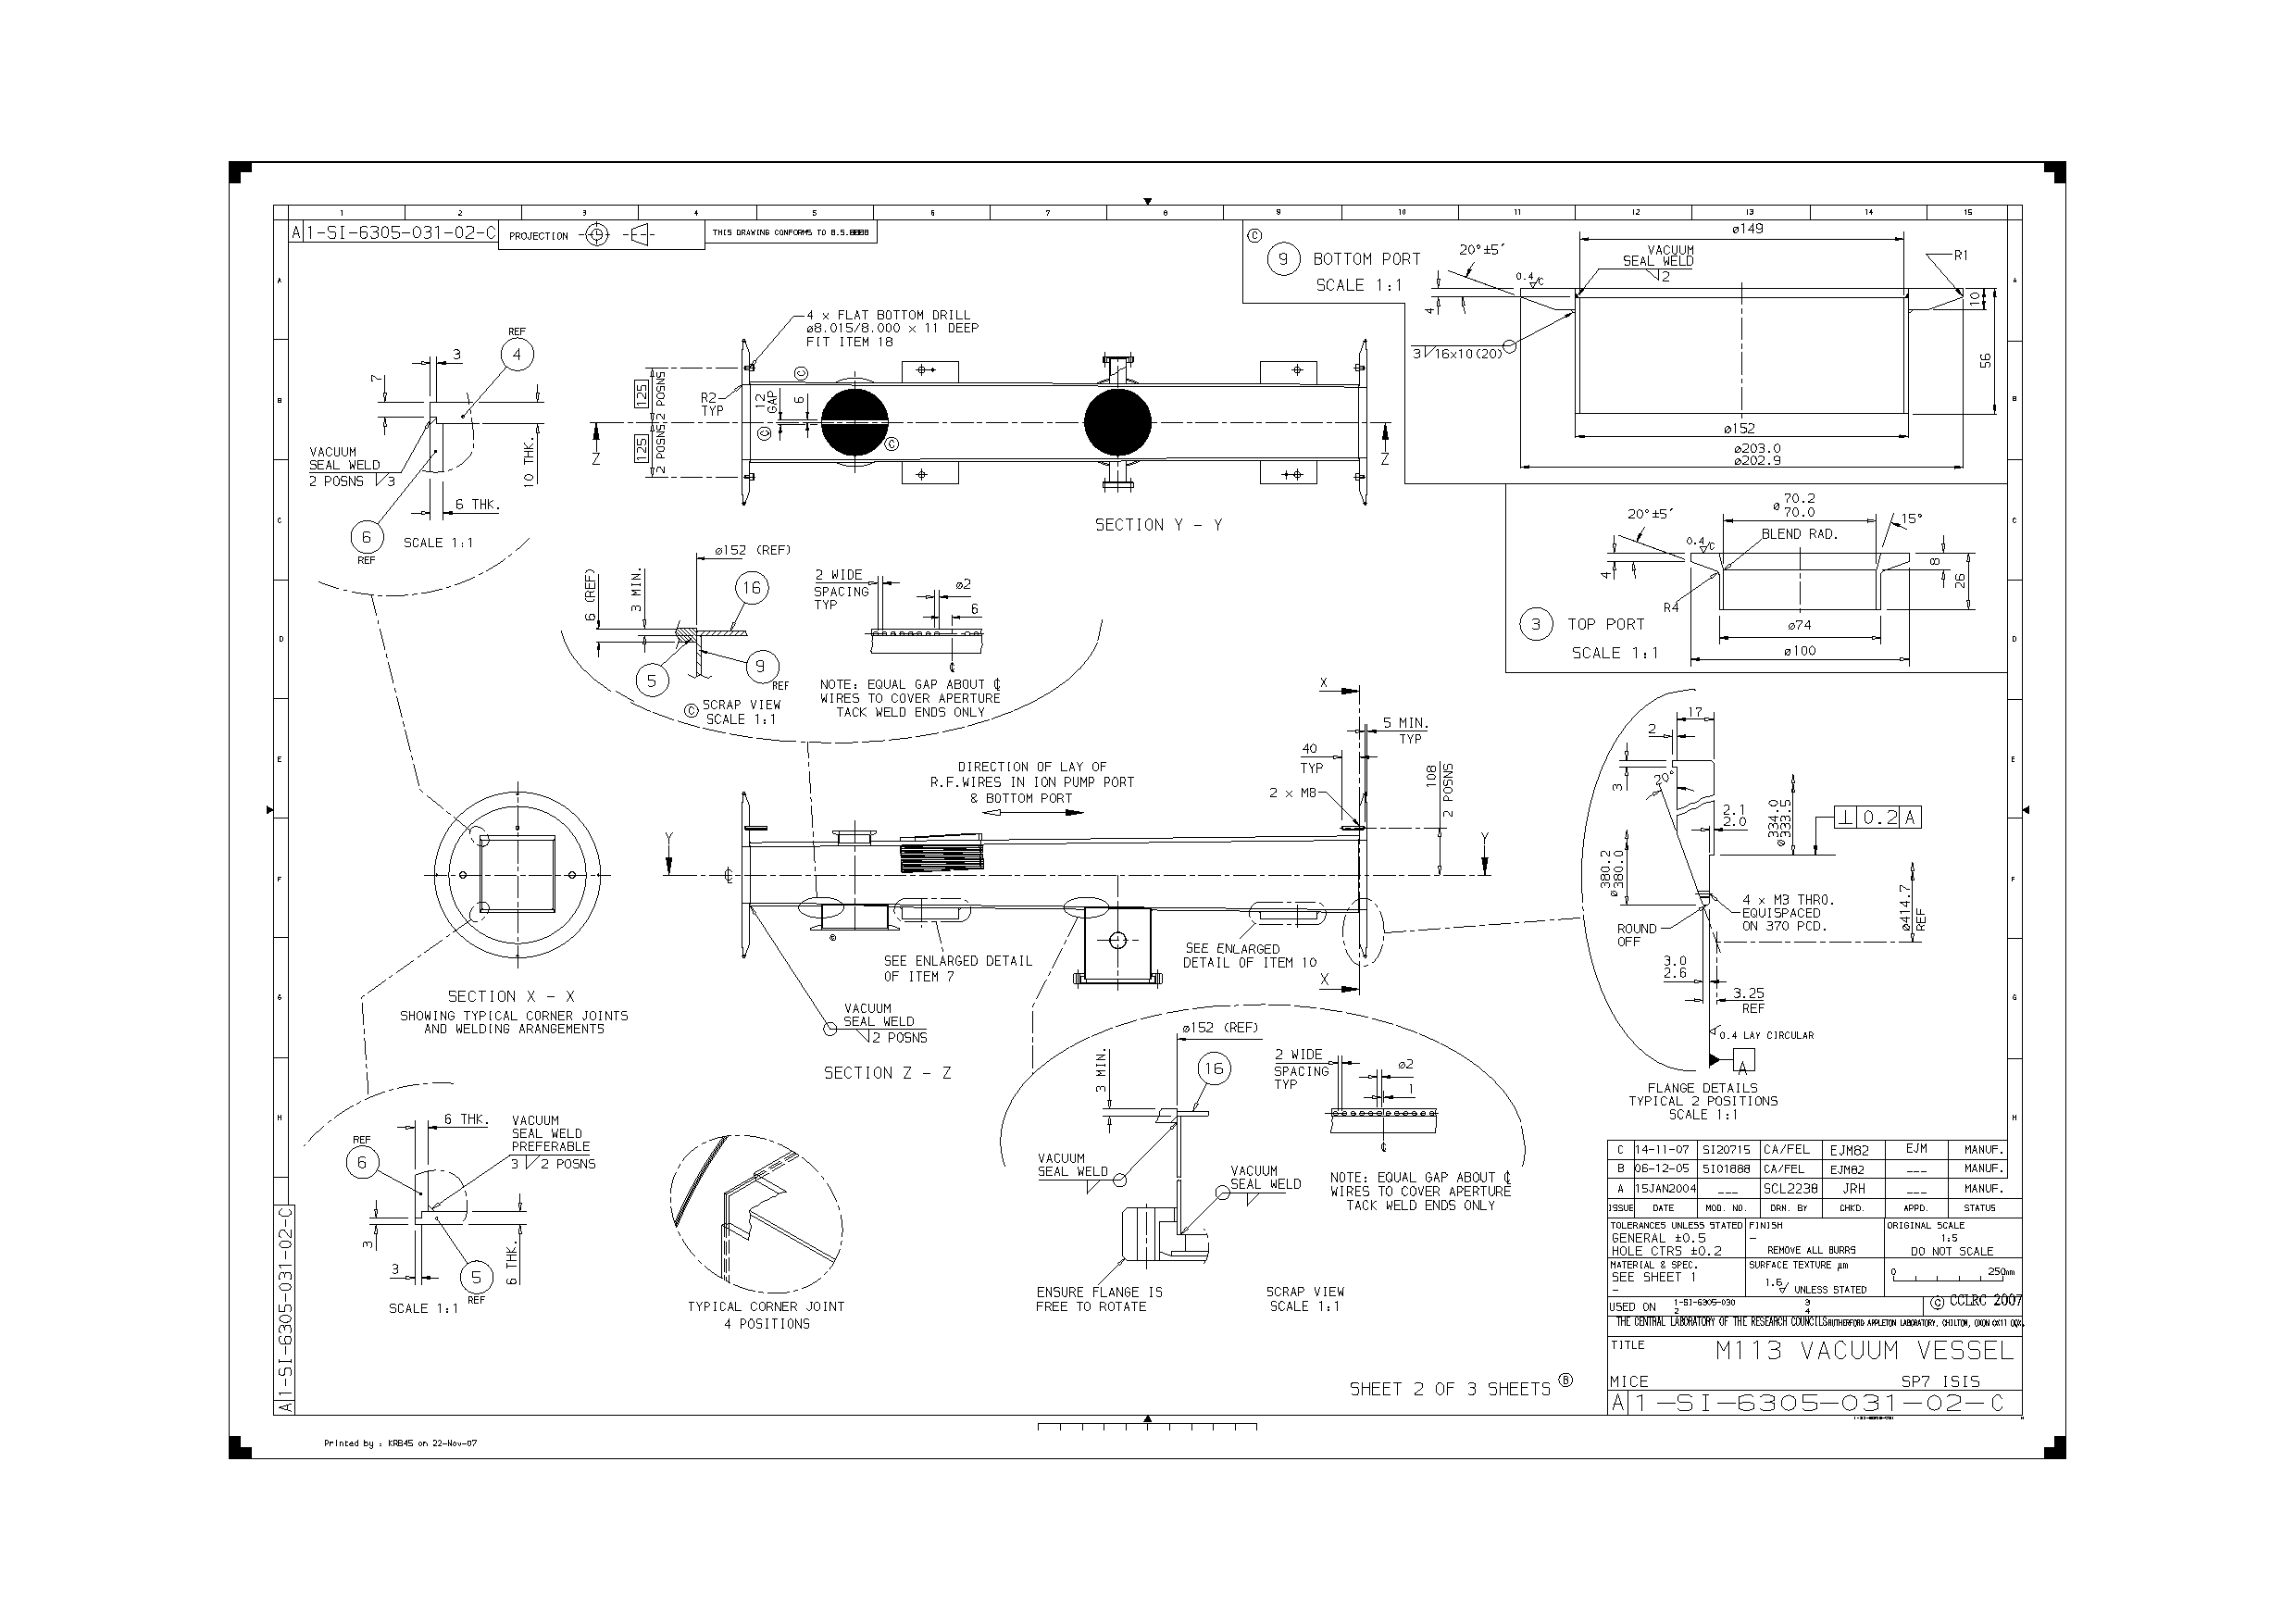
\includepdf{./figures/BeampipeSurvey2.pdf}
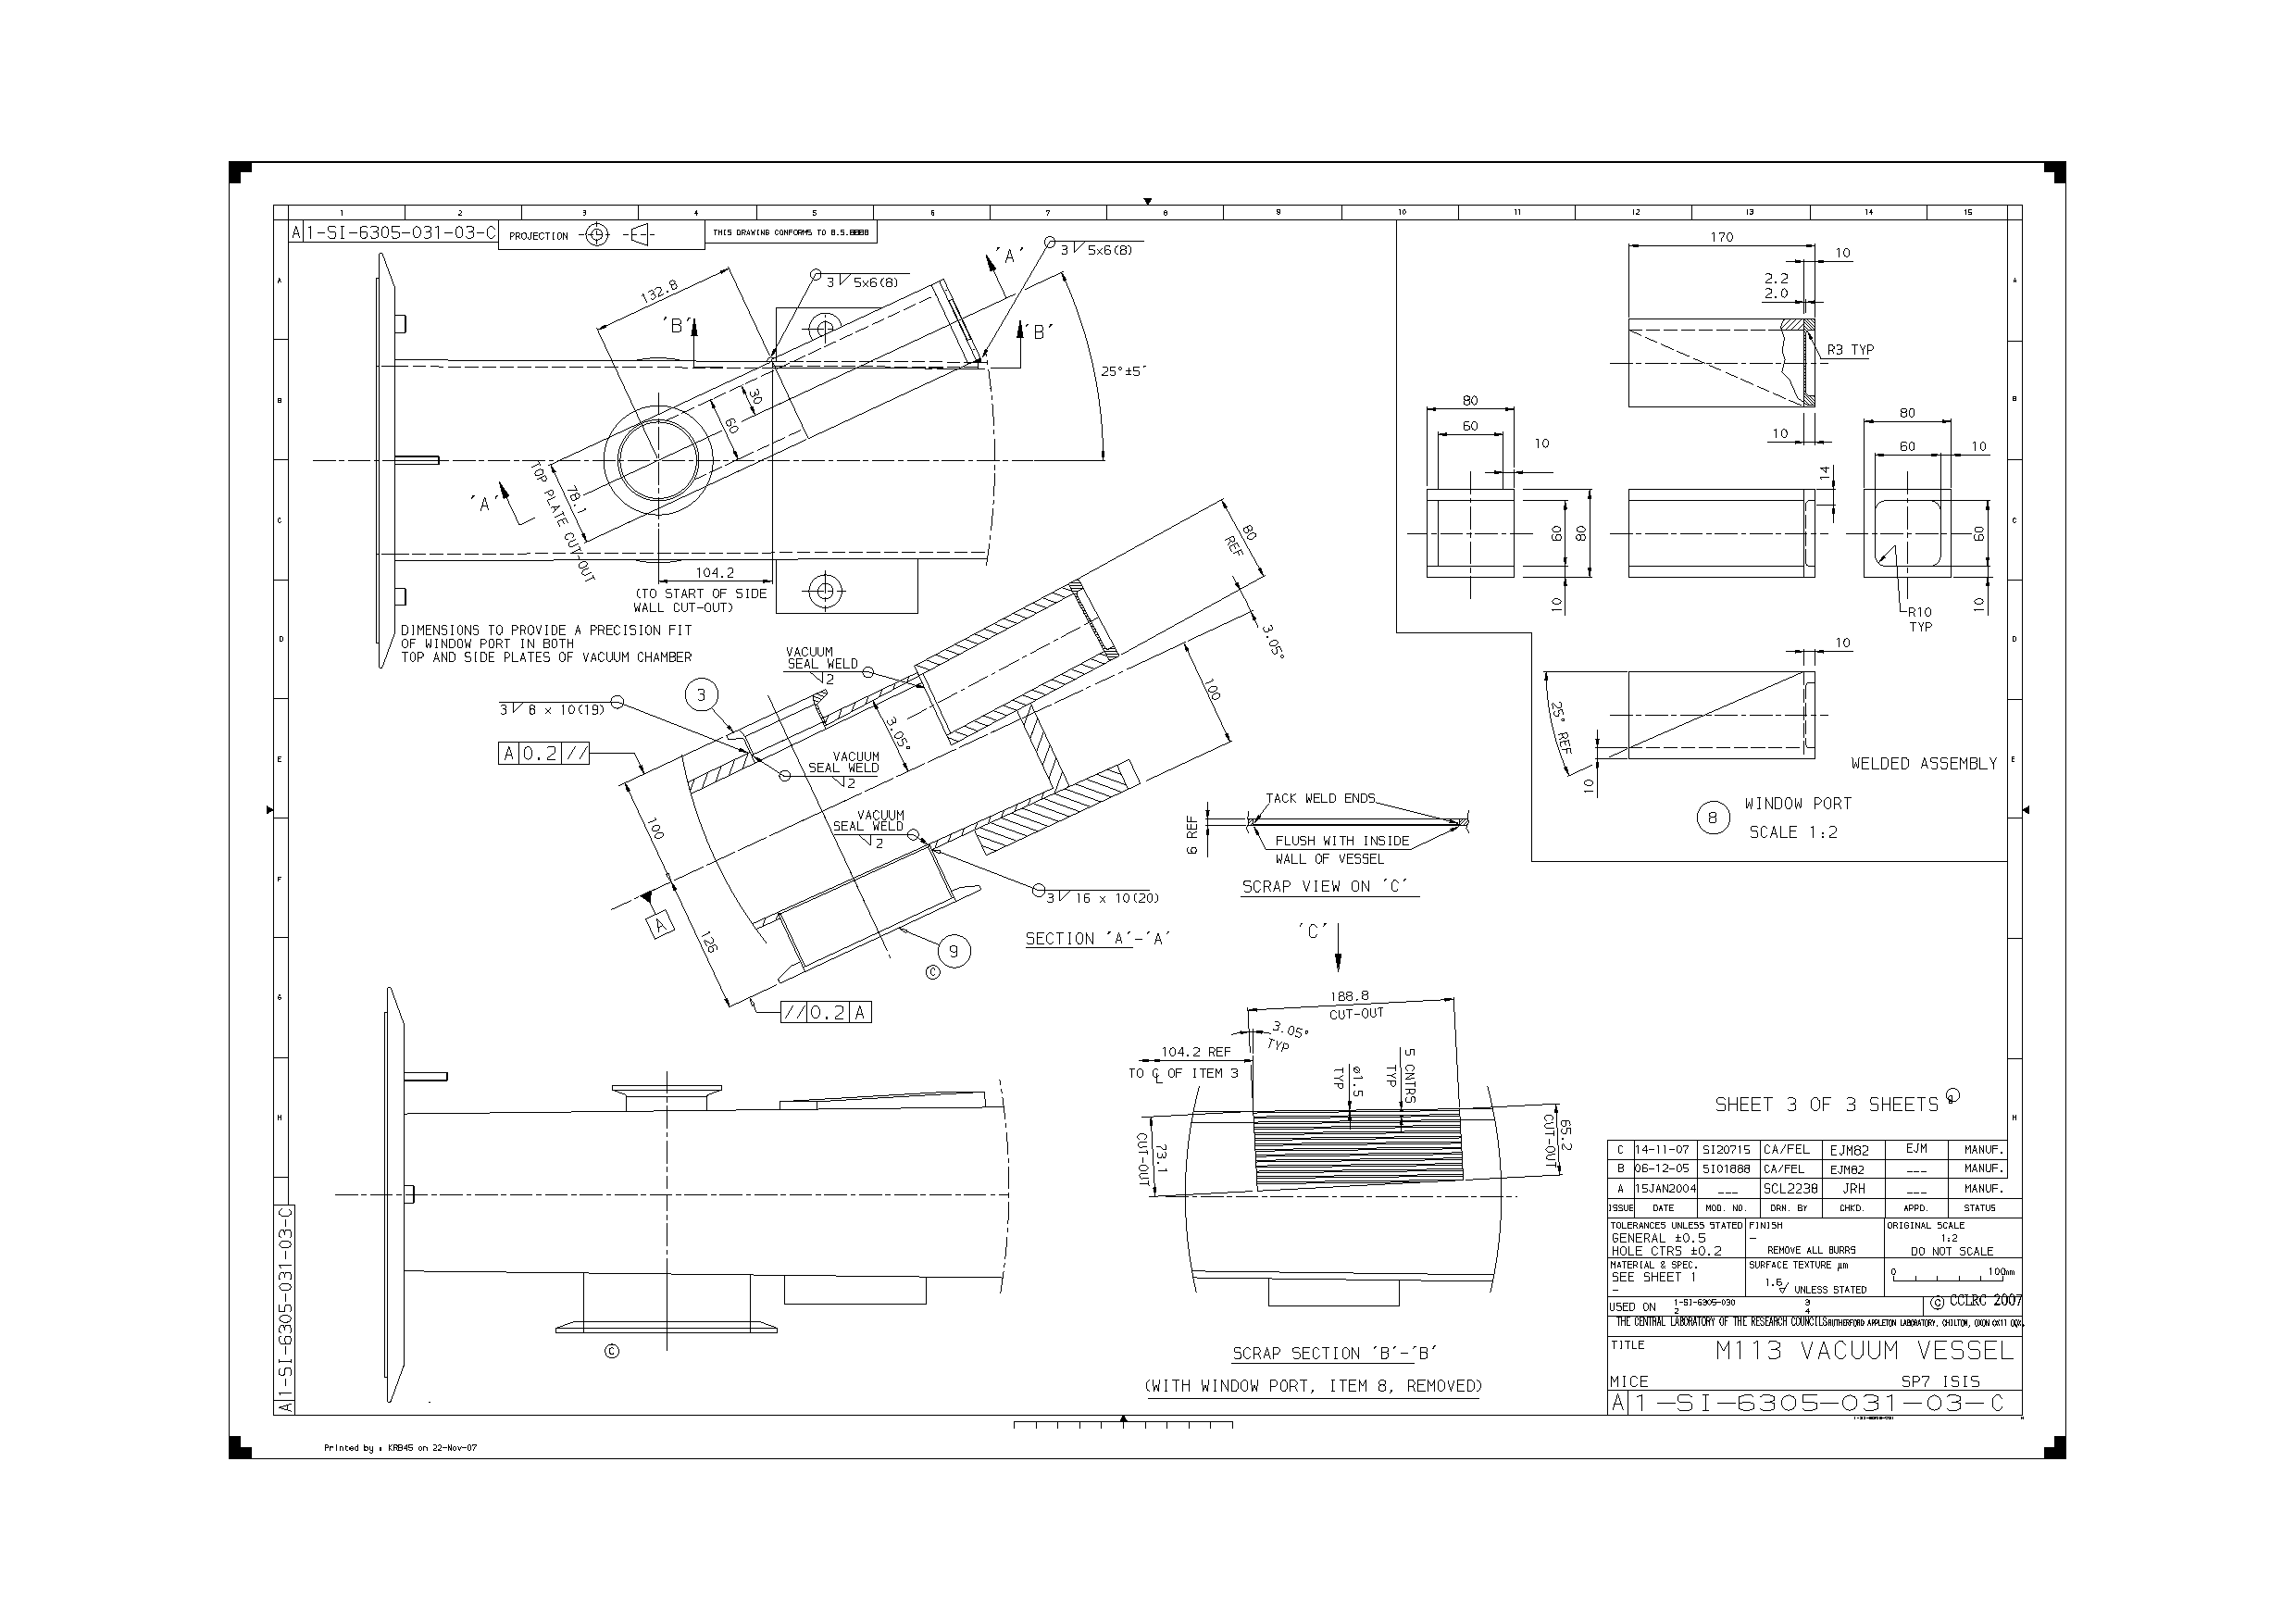
\includepdf{./figures/BeampipeSurvey3.pdf}
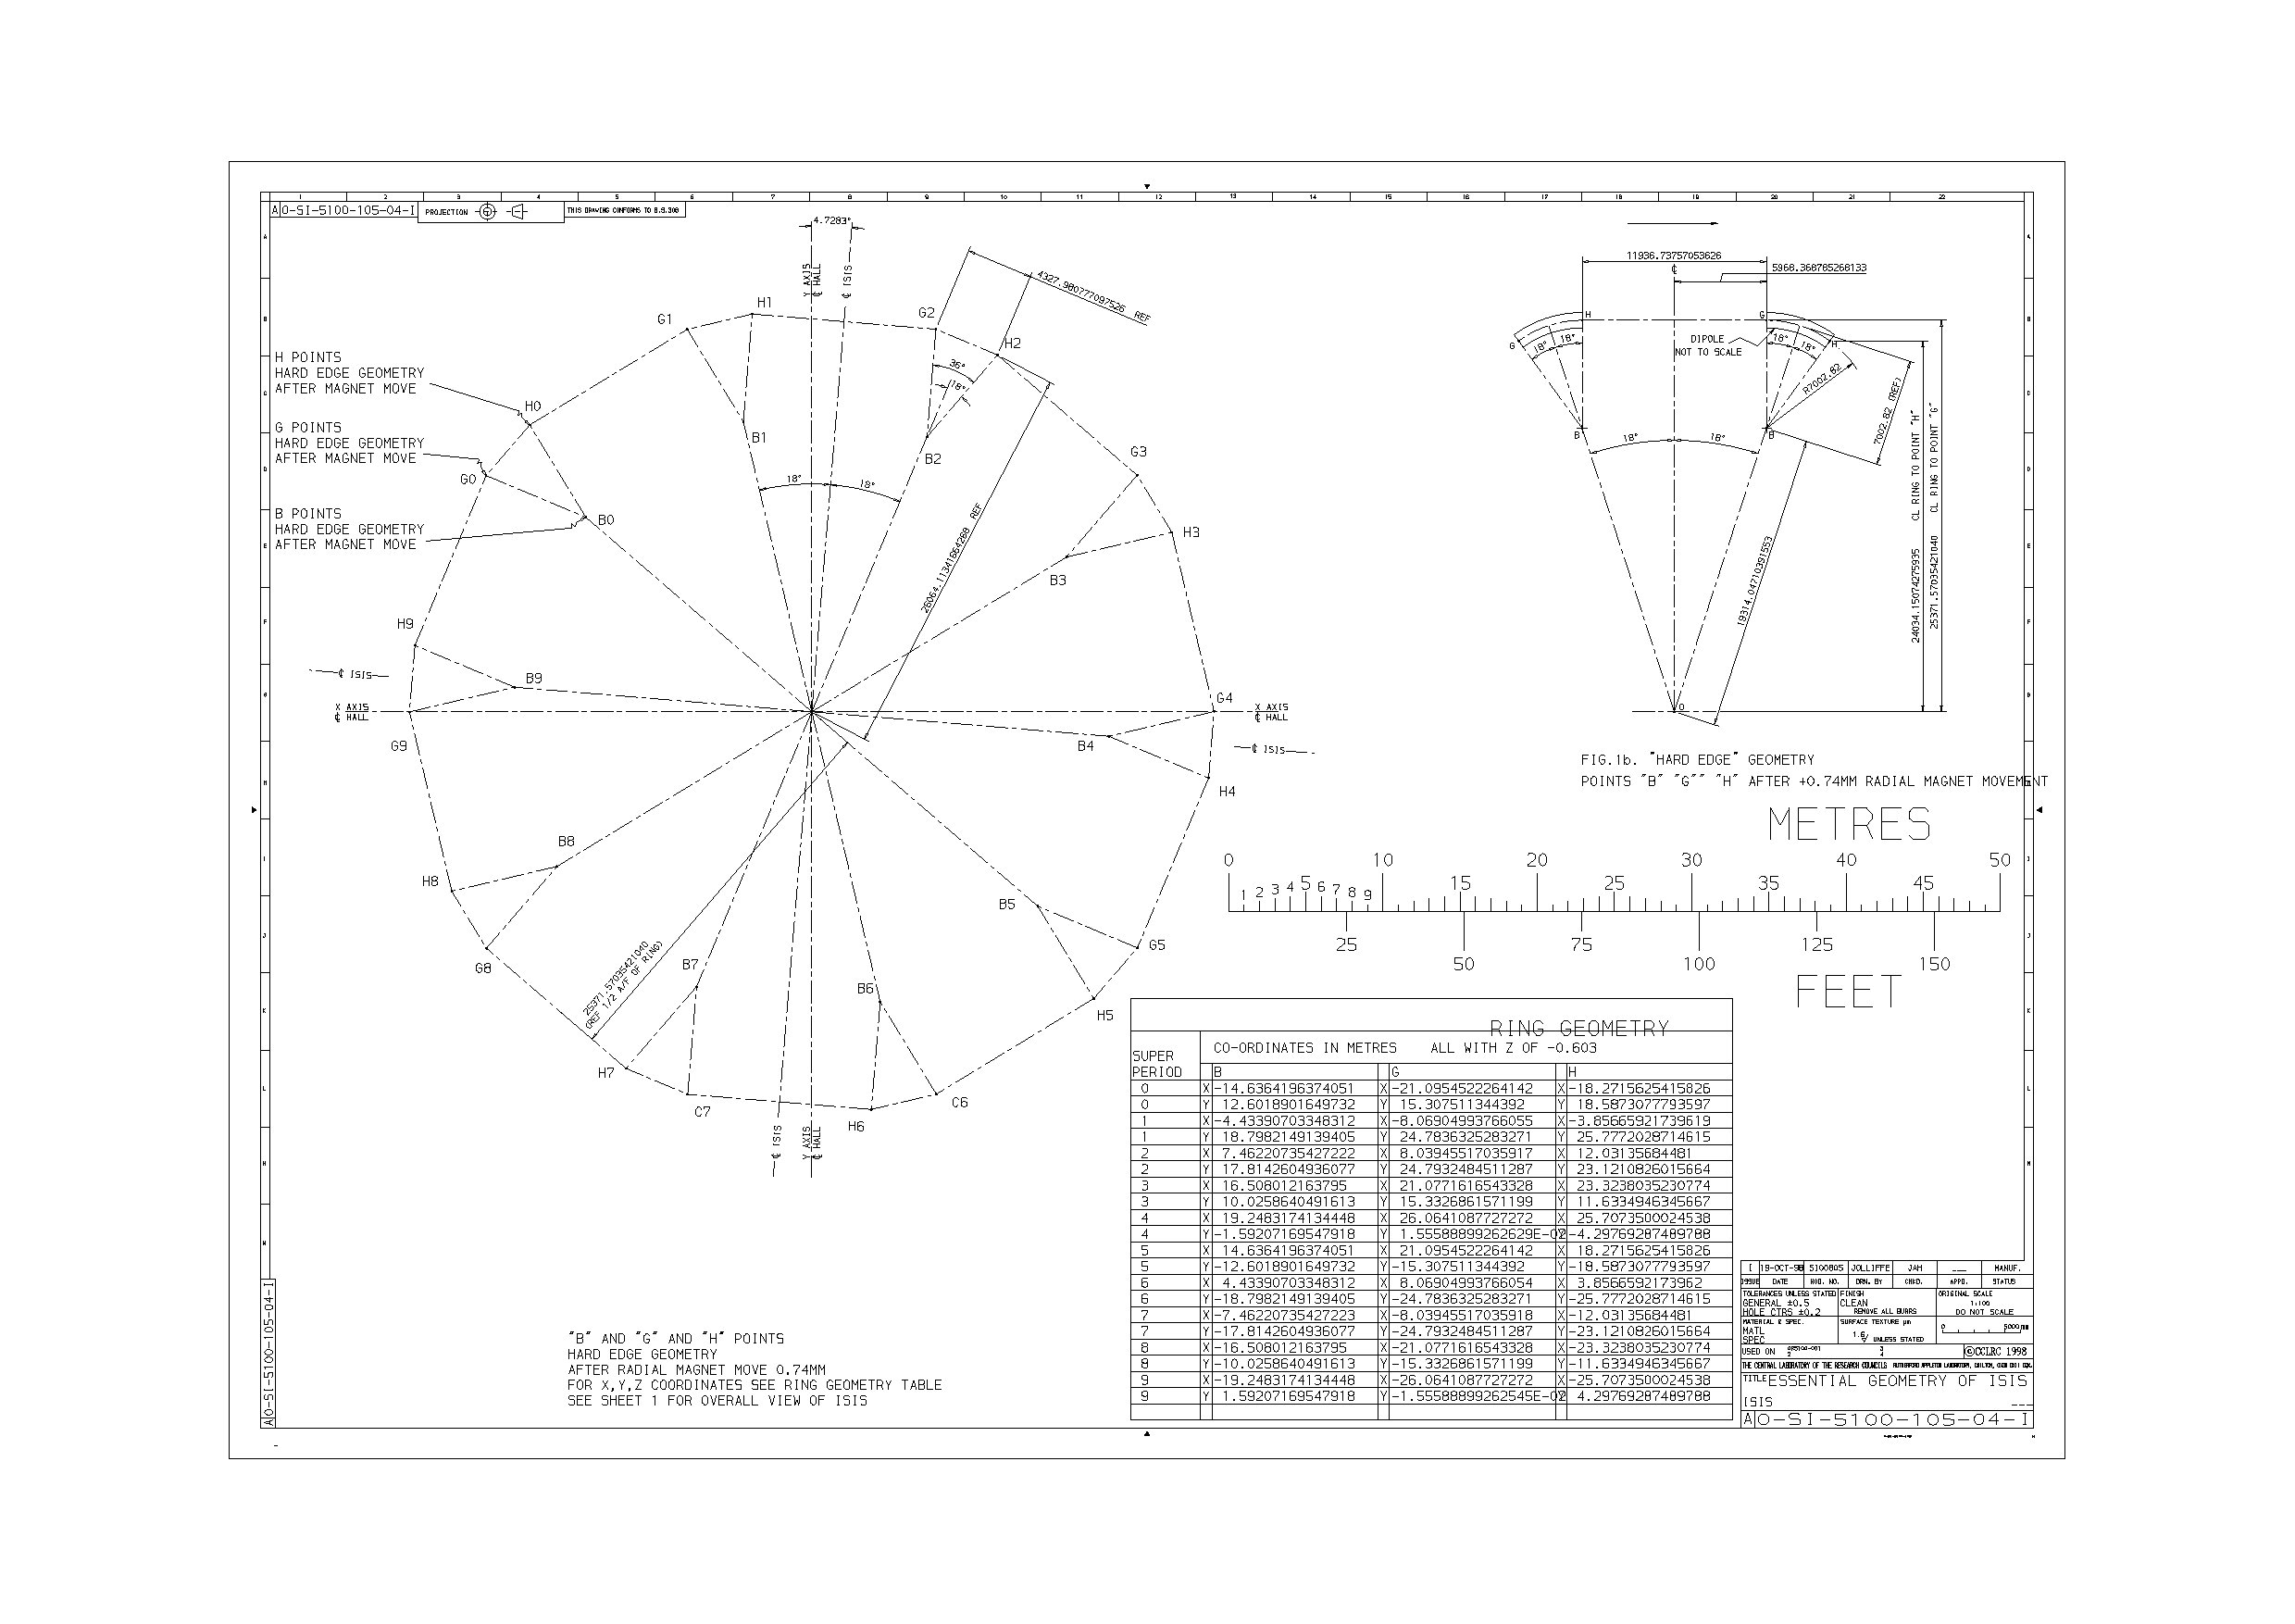
\includepdf{./figures/IsisGeometry.pdf}

\end{document}
